\section{Introducción Teórica}

Las funciones que usaremos para aproximar la inversa de la raíz son las siguientes:

\begin{displaymath}
    f(x) = x^2 - \alpha
\end{displaymath}

\begin{displaymath}
    e(x) = \frac{1}{x^2} - \alpha
\end{displaymath}

A partir de este momento nos enfocaremos en encontrar los ceros de estas dos funciones usando los métodos de Newton y de la Secante:

\begin{itemize}
    \item {\bf Newton:} $\displaystyle x_{n + 1} = x_n - \frac{h(x_n)}{h'(x_n)}$

    \item {\bf Secante:} $\displaystyle x_{n + 1} = x_{n - 1} - h(x_{n - 1})\frac{x_{n - 1} - x_{n - 2}}{h(x_{n - 1}) - h(x_{n - 2})}$
\end{itemize}

Donde $h(x) = f(x)$ o $h(x) = e(x)$ cuando corresponda 

\subsection{Análisis de $f(x)$}

Llamemos $\displaystyle \beta = \frac{1}{\alpha}$. Por otro lado la expresión de $f(x)$ la podemos reescribir de esta manera:

\begin{displaymath}
    f(x) = x^2 - \alpha = (x + \sqrt{\alpha})(x - \sqrt{\alpha})
\end{displaymath}

Estas raíces existen pues $\alpha > 0$ (pues no existe la raíz de un negativo en $\mathbb{R}$) y como podemos ver las raíces son iguales en módulo y nos sirven para hallar $\beta$ con la salvedad de que si obtenemos el valor negativo simplemente le cambiamos el signo. Por lo tanto si $\displaystyle x = \sqrt{\alpha} \implies \beta = \frac{1}{x}$\\

INSERTAR GRÁFICO DE f(x)\\

$f(x)$ es convexa y su derivada segundo es $f''(x) = 2$, al ser constante y por la
forma que tienen las derivadas asumimos que siempre va a converger.

\subsection{Análisis de $e(x)$}

\begin{displaymath}
    e(x) = 0 \implies 0 = \frac{1}{x^2} - \alpha \implies \alpha = \frac{1}{x^2} \implies x^2 = \frac{1}{\alpha}
\end{displaymath}

$e(x)$ con $\alpha > 0$ también tiene dos raíces por lo que al igual que con
$f(x)$ nos es indistinto cuál de las dos obtenemos. En este caso es importante
notar que en el 0, hay una asíntota de las ordenadas.\\

INSERTAR GRÁFICO DE e(x)
 
Los dos métodos que elegimos trabajan con la tangente de las funciones en un
punto o con una aproximación de esta.\\

Observamos $e''(x) = 6/x^4$. Esto quiere decir que la misma tiene una asíntota en el 0,
y una pendiente que se agudiza rápidamente cerca de 0, lo cual puede dificultar la convergencia,
dado que para que las operaciones aritméticas involucradas en los métodos de aproximación 
den resultados de buena precisión, dependen de trabajar con números bien representables en punto flotante.

\subsection{Convergencia}
Por lo visto en la teórica sabemos que el órden de convergencia de Newton es cuadrático, mientras que para Secante es $supralineal$ (específicamente es $\phi \approx 1.618$).

\subsubsection{Prueba de la convergencia de Newton para $f(x)$}
Vamos a demostrar inductivamente la convergencia del método de Newton usando la función $\displaystyle f(x) = x^2 - \alpha$. De esta manera la sucesión nos queda:

\begin{displaymath}
    x_{n + 1} = \frac{1}{2}(x_n + \frac{\alpha}{x_n})
\end{displaymath}

Lo que queremos demostrar es que si $x_0 > \sqrt{\alpha}$ entonces $x_{n + 1} < x_n$ para todo $n > 0$.\\

{\large \bf Inducción en k $\in \mathbb{N}$}\\
Queremos probar que $x_{k + 1} < x_k$.\\

{\bf Caso base: $P(0)$}\\
Sea $k = 1$, queremos ver que $x_1 < x_0$. Entonces reemplazando $x_1$ por su definición tenemos:

\begin{displaymath}
    \frac{1}{2}(x_0 + \frac{\alpha}{x_0}) < x_0 \iff x_0 + \frac{\alpha}{x_0} < 2x_0 \iff \frac{\alpha}{x_0} < x_0 \iff \alpha < x_0^2 \iff \sqrt{\alpha} < x_0
\end{displaymath}

Y esto último es la precondición. Por lo tanto $x_1 < x_0$ $_\square$\\

Veamos también que $x_1 > \sqrt{\alpha}$\\

\begin{displaymath}
    x_1 > \sqrt{\alpha} \iff \frac{1}{2}(x_0 + \frac{\alpha}{x_0}) > \sqrt{\alpha} \iff x_0 + \frac{\alpha}{x_0} > 2\sqrt{\alpha}
\end{displaymath}

\begin{displaymath}
    \iff x_0 - 2\sqrt{\alpha} > -\frac{\alpha}{x_0} \iff x_0^2 - 2\sqrt{\alpha}x_0 + \alpha > 0 \iff (x_0 - \sqrt{\alpha})^2 > 0
\end{displaymath}

Luego esto último vale pues $x_0 > \sqrt{\alpha}$. Por lo tanto, por esto y por lo demostrado antes vale que:

\begin{displaymath}
    \sqrt{\alpha} < x_1 < x_0
\end{displaymath}

{\bf Caso n + 1: $P(n) \implies P(n + 1)$}\\
Sea $k = n + 1$. Queremos probar que $x_{n + 1} < x_n$. Por lo visto en nuestro caso base la {\bf Hipótesis Inductiva} es:

\begin{displaymath}
    \sqrt{\alpha} < x_n < x_{n - 1}
\end{displaymath}

Entonces:
\begin{displaymath}
    x_{n + 1} = \frac{1}{2}(x_n + \frac{\alpha}{x_n}) = \frac{x_n^2 + \alpha}{2x_n}
\end{displaymath}

Luego por {\bf HI} vale que $\sqrt{\alpha} < x_n \iff \alpha < x_n^2 $ Entonces:

\begin{displaymath}
    \frac{x_n^2 + \alpha}{2x_n} < \frac{x_n^2 + x_n^2}{2x_n} = x_n
\end{displaymath}

Por lo tanto $x_{n + 1} < x_n$ $\square$


\begin{center}
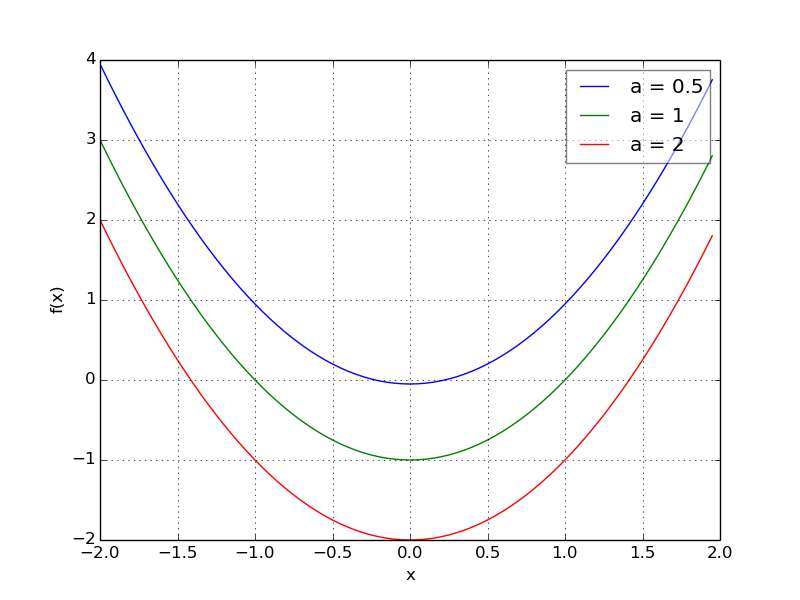
\includegraphics[scale=0.5]{graficos/f(x).png}\\
Gráfico de $f(x)$ variando $\alpha$
\end{center}

\begin{center}
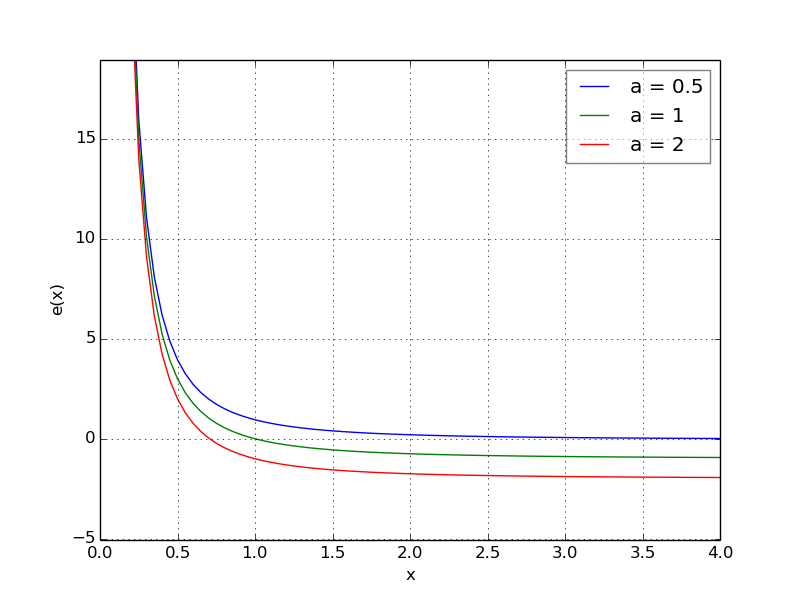
\includegraphics[scale=0.5]{graficos/e(x).png}\\
Gráfico de $e(x)$ variando $\alpha$
\end{center}
